\uuid{31dl}
\exo7id{7132}
\auteur{megy}
\organisation{exo7}
\datecreate{2017-02-08}
\isIndication{true}
\isCorrection{true}
\chapitre{Géométrie affine euclidienne}
\sousChapitre{Géométrie affine euclidienne du plan}

\contenu{
\texte{
% similitudes

On considère l'énoncé suivant :

\begin{theoreme}[Ptolémée] Soit $ABCD$ un quadrilatère convexe, direct. Alors $A, B, C, D$ sont cocycliques si et seulement si $ AC\cdot BD = AB\cdot CD + BC\cdot AD$.
\end{theoreme}

L'objectif de cet exercice est de prouver le sens direct du théorème.

On suppose $A, B, C, D$ cocycliques.
}
\begin{enumerate}
    \item \question{Faire une figure au brouillon et montrer que $\widehat{BAC} = \widehat{BDC}$ et trois relations similaires sur d'autres angles.}
    \item \question{Soit $K$ le point de la diagonale $[AC]$ tel que $\widehat{ABK} = \widehat{DBC}$. Faire une figure et construire $K$ en expliquant (faire la figure de telle sorte que $K$ soit lisible).}
    \item \question{Montrer que les triangles $ABK$ et $DBC$ sont semblables, de même que $ABD$ et $KBC$, par des similitudes dont on précisera les centres et les rapports. Note : il suffit pour cela de montrer qu'ils ont mêmes angles. En déduire des relations sur les côtés de ces triangles.}
    \item \question{Conclure.}
\reponse{
Le théorème de l'angle inscrit sur l'arc $BC$ donne l'égalité $\widehat{BAC} = \widehat{BDC}$. La considération des autres arcs $CD$, $DA$ et $AB$ donne les égalités $\widehat{DAC} = \widehat{DBC}$, $\widehat{DBA} = \widehat{DCA}$ et $\widehat{ACB} = \widehat{ADB}$.

\begin{center}
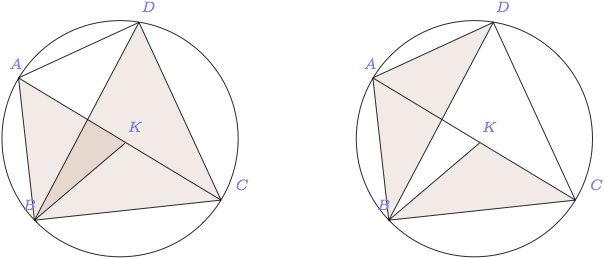
\includegraphics{../images/img007132-1}
\end{center}
 
Suivons l'énoncé. Soit $K$ le point de la diagonale $[AC]$ tel que $\widehat{ABK} = \widehat{DBC}$.

Alors,  $ABK$ et $DBC$ sont semblables (première figure) car leurs angles sont égaux :  $\widehat{BAK} = \widehat{BDC}$ et $\widehat{ABK} = \widehat{DBC}$. On a une similitude de rapport 
\[\frac{BD}{BA} = \frac{BC}{BK} = \frac{DC}{AK},\]
envoyant $ABK$ sur $DBC$.

De même, $ABD$ et $KBC$ sont semblables (deuxième figure) car leurs angles sont égaux : $\widehat{ADB} = \widehat{ACB} = \widehat{KCB}$ et $\widehat{ABD} = \widehat{KBC}$. La similitude envoyant $ABD$ sur $KBC$  a pour rapport \[\frac{BK}{BA}=\frac{BC}{BD} = \frac{KC}{AD}.\]

 


On a $AC = AK + KC$, donc $AC\cdot BD  = AK \cdot BD + KC\cdot BD$, 
or, $AK\cdot BD = AB\cdot CD$ (première similitude), et $KC \cdot BD = AD\cdot BC$ (seconde similitude), d'où le résultat:
\[ AC\cdot BD = AB\cdot CD + AD\cdot BC.\]
}
\indication{Pour la conclusion, utiliser $AC = AK + KC$.}
\end{enumerate}
}
